% https://www.overleaf.com/learn/latex/Beamer
\documentclass{beamer}

\usepackage[utf8]{inputenc}
\usepackage[T1]{fontenc}
\usepackage[slovene]{babel}
\usepackage{lmodern}
\usepackage{array}
\usepackage{tikz}

\usepackage{hyperref}

\usetheme{Berlin}
\usecolortheme{default}
\useinnertheme[shadows]{rounded}
\useoutertheme{infolines}
% \beamertemplatenavigationsybolsempty

\usepackage{palatino}
\usefonttheme{serif}

\newtheorem{definicija}{Definicija}
\newtheorem{izrek}{Izrek}

\title{Priprava prosojnic v \LaTeX-u}
\subtitle{Uporaba paketa beamer}
\author{Matic Zavadlal}
\institute[FMF]{FMF Fakulteta za matematiko in fiziko}

\begin{document}

% ===================================================================

\begin{frame}
   \titlepage
\end{frame}

% -------------------------------------------------------------------

\begin{frame}

\frametitle{Kratek pregled}
\tableofcontents[pausesections]

\end{frame}

% -------------------------------------------------------------------

\section{Razporeditev vsebine}

\begin{frame}
   \frametitle{Naštevanje}
   
   Za naštevanje lahko uporabimo okolje itemize:
   \begin{itemize}
      \item<1-> Prva točka.
      \item<2-> Druga točka.
      \item<3-> Tretja točka.
   \end{itemize}
   ali pa okolje enumerate:
   \begin{enumerate}
      \item<4-> Prva točka.
      \item<5-> Druga točka.
      \item<6-> Tretja točka.
   \end{enumerate}

\end{frame}
% -------------------------------------------------------------------

\begin{frame}
   \frametitle{Bloki z naslovom}

   Dele besedila lahko zapišemo v bloke.
   Uporabimo okolja block, exampleblock, alertblock.
   Za parameter okolja napišemo naslov bloka.

   \begin{block}{Opomba}
      Tako je videti block z naslovom.
   \end{block}
   
   \begin{examples}{Primer}
      Tako je videti exampleblock z naslovom.
   \end{examples}

   \begin{alertblock}{Opozorilo}
      Tako je videti alertblock z naslovom.
   \end{alertblock}

\end{frame}

% -------------------------------------------------------------------

\begin{frame}
   \frametitle{Bloki brez naslova}

   Blok lahko ima tudi prazen naslov.
   
   V takem primeru bo brez naslovne vrstice.
   \begin{block}{}
      Tako je videti block s praznim naslovom.
   \end{block}
   \begin{exampleblock}{}
      Tako je videti exampleblock s praznim naslovom.
   \end{exampleblock}
   \begin{alertblock}{}
      Tako je videti alertblock s praznim naslovom.
   \end{alertblock}
\end{frame}

% -------------------------------------------------------------------

\begin{frame}
   \frametitle{Stolpci}


   \begin{columns}
      \begin{column}{0.5\textwidth}
         Besedilo lahko pišemo v več stolpcih.
         Osnovno okolje je columns.
         Posamezen stolpec opišemo v okolju column.
         Vsebina stolpca je lahko poljubna.
         Za primer imamo v desnem stolpcu napis v bloku in sliko sončnice.
      \end{column}

      % https://tex.stackexchange.com/questions/9464/beamer-text-and-image-on-the-same-slide#9468xtwidth}
      \begin{column}{0.5\textwidth}
         \begin{block}{}
            Slika v stolpcu
         \end{block}

         \includegraphics[width=\textwidth]{soncnica.jpg}
      \end{column}
   \end{columns}
\end{frame}

% ===================================================================

\section{Matematične trditve}

% -------------------------------------------------------------------

\begin{frame}
   \frametitle{Praštevila}

   % https://tex.stackexchange.com/questions/233129/theorem-boxes-in-beamer#233184
   \begin{definicija}
      Praštevilo je naravno število, ki ima natanko dva delitelja.
   \end{definicija}

   \begin{examples}{Zgledi}
      \begin{itemize}
         \item 1 je praštevilo (ima samo enega delitelja: 1).
         \item 2 je praštevilo (ima dva delitelja: 1 in 2).
         \item 3 je praštevilo (ima dva delitelja: 1 in 3).
         \item 4 ni praštevilo (ima tri delitelje: 1, 2 in 4).
      \end{itemize}
   \end{examples}

\end{frame}



% -------------------------------------------------------------------

\begin{frame}
   \frametitle{Praštevila}

   \begin{izrek}
      Praštevil je neskončno mnogo.
   \end{izrek}

   \begin{proof}
      Denimo, da je praštevil končno mnogo.
         Naj bo p največje praštevilo.
         Naj bo q produkt števil 1, 2, ??, p.
         Število q+1 ni deljivo z nobenim praštevilom, torej je q+1 praštevilo.
         To je protislovje, saj je q+1>p.
   \end{proof}

\end{frame}

% ===================================================================

\section{Postopno odkrivanje vsebine}

% -------------------------------------------------------------------
\begin{frame}
   \frametitle{Konstrukcija pravokotnice na premico p skozi točko T}
   \begin{columns}
      \begin{column}{0.55\textwidth}
         \begin{itemize}
            \item<1->Dani sta premica p in točka T.
            \item<2->Nariši lok k s središčem v T.
            \item<3->Premico p seče v točkah A in B.
            \item<4->Nariši lok m s središčem v A.
            \item<5->Nariši lok n s središčem v B in z enakim polmerom.
            \item<6->Loka se sečeta v točki C.
            \item<7->Premica skozi točki T in C je pravokotna na p.
         \end{itemize}
      \end{column}

      \begin{column}{0.45\textwidth}
         \centering
         \includegraphics<1>[width=\textwidth]{pic1.png}
         \includegraphics<2>[width=\textwidth]{pic2.png}
         \includegraphics<3>[width=\textwidth]{pic3.png}
         \includegraphics<4>[width=\textwidth]{pic4.png}
         \includegraphics<5>[width=\textwidth]{pic5.png}
         \includegraphics<6>[width=\textwidth]{pic6.png}
         \includegraphics<7>[width=\textwidth]{pic7.png}
      \end{column}
   \end{columns}

\end{frame}

% -------------------------------------------------------------------

\begin{frame}
   \frametitle{Odkrivanje tabele po vrsticah}

   \begin{tabular}{c|*4{c}}
         Oznaka & A & B & C & D \\ \hline
         \onslide<1->{X & 1 & 2 & 3 & 4} \\
         \onslide<2->{Y & 3 & 4 & 5 & 6} \\
         \onslide<3->{Z & 5 & 6 & 7 & 8}
   \end{tabular}

\end{frame}

% -------------------------------------------------------------------

\begin{frame}
   \frametitle{Odkrivanje tabele po stolpcih}

   \begin{tabular}{c | >{\onslide<2->}c >{\onslide<3->}c >{\onslide<4->}c >{\onslide<5->}c <{\onslide}}
      Oznaka & A & B & C & D \\ \hline
      X & 1 & 2 & 3 & 4 \\
      Y & 3 & 4 & 5 & 6 \\
      Z & 5 & 6 & 7 & 8
   \end{tabular}
   
\end{frame}

% ===================================================================

\section{Razno}

% -------------------------------------------------------------------

\begin{frame}
   \centering
   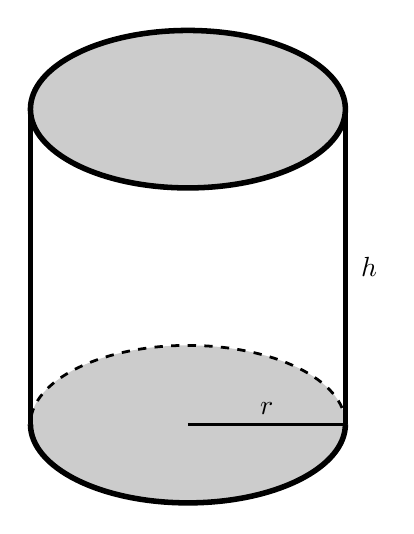
\begin{tikzpicture}
      \onslide<3->
      \begin{scope}[color=black!20]
         \fill (0,4) circle [x radius=2, y radius=1];
         \fill (0,0) circle [x radius=2, y radius=1];
      \end{scope}

      \onslide<2->
      \draw[black, line width=2pt] (-2,0) -- (-2,4);
      \draw[black, line width=2pt] (2,0) -- (2,4);
      \draw[black, line width=2pt] (0,4) ellipse [x radius=2, y radius=1];
      \draw[black, line width=2pt] (-2,0) arc [start angle=180, end angle=360, x radius=2, y radius=1];

      \onslide<3->
      \draw[black, line width=1pt, dashed] (2,0) arc [start angle=0, end angle=180, x radius=2, y radius=1];

      \onslide<4->
      \node at (1,0.2) {$r$};
      \node at (2.3,2) {$h$};
      \draw[black, line width=1pt] (0,0) -- (2,0);

   \end{tikzpicture}

\end{frame}

% ===================================================================

\end{document}